\begin{solutionbox}[Q3-1]

    \begin{center}
        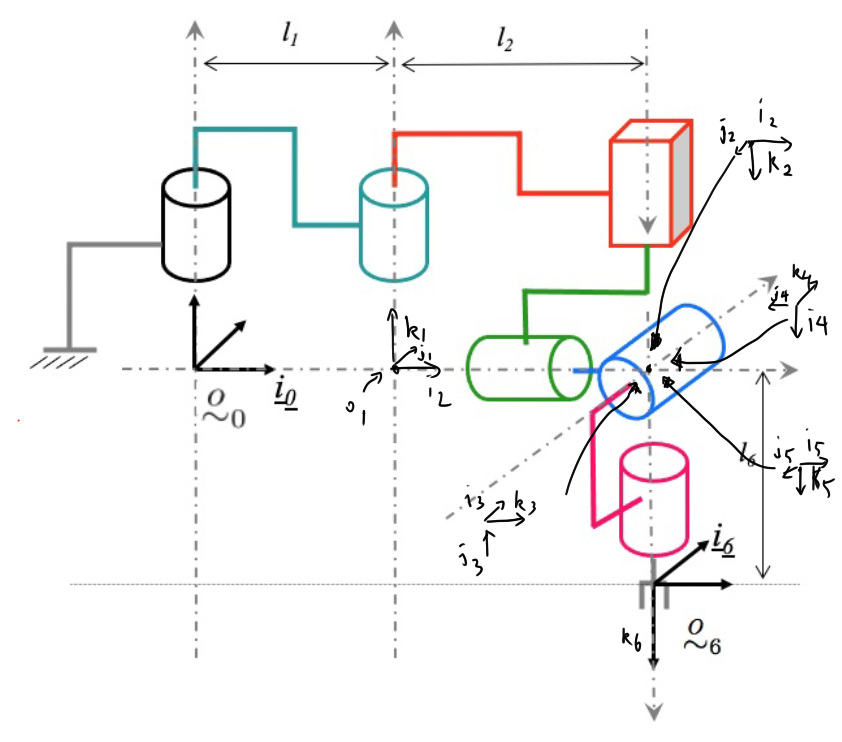
\includegraphics{imgs/y2022-v1-q3-1.png}
    \end{center}

    I don't think I actually need to generate DH table for this?

    Coordinate free form, very standard axis.

    Singularity when $\theta_2=0$ or $\pi$ which is elbow singularity. And when $\theta_5 =\pi/2$ or $3\pi/2$ which is a wrist singularity
\end{solutionbox}

\begin{solutionbox}[Q3-2]
    Walk back from o6 by k3 l6 to find o3.

    Project o3-o0 to plane perpendicular to k3.

    Use Kahan p4 to find theta 2 and theta 1. There is a branching here.

    Project o3-o0 onto k3, this is d3.

    With first three, C3 is known.

    $\pv{k}_4 = \pm \pv{k}_3\times \pv{k}_6 k4$ There is branching here.

    Use Kahan p2 to rotate i3 to k4 through k3 gives theta 4.

    Use Kahan p2 to rotate i4 to k5 through k4 gives theta 5.

    Use Kahan p2 to rotate i5 to j6 though k5 gives theta 6.

\end{solutionbox}